\documentclass[a4paper, 11pt]{report}
\usepackage{blindtext}
\usepackage[T1]{fontenc}
\usepackage[utf8]{inputenc}
\usepackage{titlesec}
\usepackage{fancyhdr}
\usepackage{geometry}
\usepackage{fix-cm}
\usepackage[hidelinks]{hyperref}
\usepackage{graphicx}

\usepackage[english]{babel}

\graphicspath{ {./images/} }
\geometry{ margin=30mm }
\counterwithin{subsection}{section}
\renewcommand\thesection{\arabic{section}.}
\renewcommand\thesubsection{\thesection\arabic{subsection}.}
\usepackage{tocloft}
\renewcommand{\cftchapleader}{\cftdotfill{\cftdotsep}}
\renewcommand{\cftsecleader}{\cftdotfill{\cftdotsep}}
\setlength{\cftsecindent}{2.2em}
\setlength{\cftsubsecindent}{4.2em}
\setlength{\cftsecnumwidth}{2em}
\setlength{\cftsubsecnumwidth}{2.5em}

\newenvironment{boldbox}
    {\begin{center}
    \begin{tabular}{|p{0.9\textwidth}|}
    \hline\\
    \bfseries
    }
    { 
    \\\\\hline
    \end{tabular} 
    \end{center}
    }


\begin{document}
\titleformat{\section}
{\normalfont\fontsize{15}{0}\bfseries}{\thesection}{1em}{}
\titlespacing{\section}{0cm}{0.5cm}{0.15cm}
\titleformat{\subsection}
{\normalfont\fontsize{13}{0}\bfseries}{\thesubsection}{0.5em}{}
\titlespacing{\section}{0cm}{0.5cm}{0.15cm}

%=======================================================================================

% #########################
% IMPORTANT - Add student names here!
% e.g. \newcommand{\stud1}{LOWE, David}
\newcommand{\studA}{{BLIGHT, Matthew}}
\newcommand{\studB}{{LOUIS, Tobit}}
\newcommand{\studC}{{TRAN, Jordan}}
\newcommand{\studD}{{DANG, Chloe}}
%
% IMPORTANT - Then give your SIDs
\newcommand{\sidA}{{490423105}}
\newcommand{\sidB}{{530487713}}
\newcommand{\sidC}{{530503851}}
\newcommand{\sidD}{{530476094}}
%
% IMPORTANT - And then update which major each student will focus on
\newcommand{\majA}{{Computer Science}}
\newcommand{\majB}{{Data Science}}
\newcommand{\majC}{{SW Development}}
\newcommand{\majD}{{Cyber Security}}
% #########################


\pagenumbering{Alph}
\begin{titlepage}
\begin{flushright}

\includegraphics[width=4cm]{USyd}\\[2cm]
\end{flushright}
\center 
\textbf{\huge INFO1111: Computing 1A Professionalism}\\[0.75cm]
\textbf{\huge 2023 Semester 1}\\[2cm]
\textbf{\huge Skills: Team Project Report}\\[3cm]

\textbf{\huge Submission number: 1}\\[0.75cm]
\textbf{Github link: https://github.sydney.edu.au/mbli9416/INFO1111\_CC15\_05}\\[0.75cm]
\textbf{\huge Team Members:}\\[0.75cm]

\begin{tabular}{|p{0.25\textwidth}|p{0.13\textwidth}|p{0.12\textwidth}|p{0.12\textwidth}|p{0.22\textwidth}|}
	\hline
	Name & Student ID & \raggedright{Levels already achieved} & \raggedright{Levels being attempted} & Selected Major \\
	\hline
	\hline
	\raggedright{\studA} & \sidA & A, B & C & \majA \\
	\raggedright{\studB} & \sidB & X & A & \majB \\
	\raggedright{\studC} & \sidC & A & B,  C & \majC \\
	\raggedright{\studD} & \sidD & A & A , B & \majD \\
	\hline
\end{tabular}
\thispagestyle{empty}
\end{titlepage}
\pagenumbering{arabic}


%=======================================================================================

\tableofcontents


%=======================================================================================

\newpage
\section{Teamwork}
\label{sect-team}


\subsection{Developing industry skills}

To be trained/assisted by people who are well versed in new areas you are interested in proves to be an invaluable means of enriching your learning, given explanations are tailored to the individual and far more engaging than online courses. These people are inclusive of your superiors, coworkers or other members of your network. This approach is most appropriate once a basic understanding of the topic has been attained and you wish to master it whilst challenging yourself by developing complex projects and solving advanced problems. In this way, help is individualised and readily available. For instance, taking initiative to request and negotiate with a co-worker experienced in the field of interest for assistance - not only do they know real world applications, but also offer extensive knowledge to deepen your own understanding.

Online study courses are most appropriate for when someone wants to gain a comprehensive understanding of the programming language or topic in general. They offer the learner the opportunity to develop employable skills through the convenience of an online interface and even gain qualifications. They do however require an extensive amount of time and dedication to complete and therefore, may not be suitable for beginner programmers looking to extract quick and easy solutions as the information in these courses is often embedded amongst modules, or behind other boundaries such as having to complete previous tasks. Thus the online study courses are suitable for those willing to undertake a complete overview of a program.

Practical coding by trial-and-error, in conjunction with google (i.e. stack overflow), is another effective approach that all programmers despite their respective field or level should use for their continuous learning. Coding by trial-and-error is absolutely necessary if a programmer strives to develop new skills and proficiency in arising programming languages. This approach enables a more advanced level of skill honing, problem-solving and analysis skills to debug errors successfully (via research and google) and develop logically complex programs. Learning by trial-and-error serves as an effective method to ease into and understand all the nuanced syntaxes of a programming language. However, the method usually takes an extensive amount of time to work at before a programmer could see success for employability qualifications. Thus, this approach in conjunction with google / stack overflow is an essential part of continuous learning for programmers to hone their skills within their respective fields.

Watching educational YouTube videos is a useful approach for learning a new tool or language. Coding tutorials and other similar videos give a great foundation for understanding the workflow of the program. This can be a helpful place to start when the tool is completely foreign, as you get to see just what it looks like to use the tool in an effective way. The downside to this approach is that learners can get stuck just watching people use the tool, rather than practically using the tool themselves. The best way to gain proficiency in a skill is to acquire experience doing it. Therefore, if a programmer is neglecting to combine practical applications with the YouTube tutorials they watch, they will fail to truly make any progress in their learning and proficiency.

A final approach that can be brought to continual learning is reading the official documentation for whichever tool is being learned. While documentation can be an effective tool as a reference to understand the framework of a program, it is not very practical for learning new languages when used on its own. Programming documentation often goes into much more detail than is necessary for a basic understanding, and can be hard to decipher due to the jargon being used. It is difficult to master reading on its own, hence it is best used alongside other resources or when encountering problems in implementation. Overall, reading programming documentation on its own is not a very effective approach to learning a programming language or tool, but can be useful if a learner gets stuck on their journey.


\subsection{Submission 1 contribution overview}

After initially receiving the group project, the team discussed various strategies to evenly split the tasks presented within the Teamwork section 1.1. We concluded it was best to brainstorm five of the approaches to continual learning together, and then assign each member to complete one. Given our team comprises four members, we took initiative to complete the remaining approach during a group meeting. As for individual level A attempts, all members were able to complete their section and pull/commit changes successfully. Within the final group meeting, we finalised and ensured the TEX file contained all necessary changes. Overall, there were equal contributions and a productive work flow between members.

\subsection{Submission 2 contribution overview}

For our second submission, we started by discussing the feedback from our first submission and applying the relevant changes. Each of us made our own individual contributions through GitHub in our own time. Overall there was an equal contribution between members.

\subsection{Submission 3 contribution overview}

For our third and final submission, we began by choosing our topics so that we didn't overlap. Then we each made individual contributions in our own time through GitHub. All members contributed equally to this assignment.


%=======================================================================================

\newpage
\section{Level A: Basic Skills}

Level A focuses on basic technical skills (related to \LaTeX\ and Git) and the types of skills used in different computing jobs. Each member of the team should individually complete their subsection below. You should begin by allocating to each team member a different major to focus on (i.e. one of: Computer Science; Data Science; Software Development; Cyber Security). \textit{If you have a fifth member, then your tutor will suggest a fifth topic to cover}. This allocation should be specified above (see lines 36-55 in the LaTeX file).

You should then begin by looking at the list of skills identified within SFIA (Skills Framework for the Information Age)~\cite{sfia}. Then select two skills from the complete list:
\begin{enumerate}
	\item The skill in which you believe you are currently the strongest and which is relevant to the major you have selected. You should explain why this skill is necessary for that major, and what evidence you currently have that demonstrates your strength in this area. (Target = 200-400 words).
	\item The skill in which you believe you are currently the weakest but which is important to the major you have selected. You should explain why this skill is necessary for that major, and what you can do to improve your capability in this area. (Target = 200-400 words).
\end{enumerate}

You will need to integrate your information into the shared collaborative LaTeX document and compile the result.

\subsection{Skills for \majA: \studA}

\subsubsection{Strongest Skill: Emerging Technology Monitoring \cite{sfia}}

The ability to regularly monitor for new and emerging technologies is an invaluable skill within the field of computer science. Staying on top of new tools and techniques can help computer scientists solve problems and work more efficiently. For example, a newly developed programming language could help developers create new software at a quicker pace, or with fewer bugs.

Maintaining pace with the languages and frameworks of today can also assist in effective collaboration and communication between peers. It is much easier for computer scientists to create new software and share meaningful ideas about the future with their colleagues when they are all on the same page about the newest developments in the field. 

Moreover, having an up-to-date knowledge on current technological advancements could help computer scientists predict future trends in the industry. Today’s digital landscape is rapidly changing, with evermore products, programming languages and methodologies being developed everyday. As these new technologies become accessible, it is vital that computer scientists keep their fingers on the pulse so that they can maintain a competitive advantage in their field.

I have chosen this skill as my strongest skill that relates to the field of Computer Science, as I have a keen interest in being aware of recent developments in technology and research. I love to read online articles and consume many other resources in order to understand the newest technologies and changes in the industry. For example, when as soon as OpenAI publicly released ChatGPT, I was incredibly interested in how this technology worked, and spent time researching the implications that it and other generative AI models would have for the industry and society at large. While I do feel that I have a strength in this skill, there are still many advancements I could make such as subscribing to a daily/weekly email outlining the newest technological developments in particular fields.

\subsubsection{Weakest Skill: Scientific Modelling \cite{sfia}}

Scientific modelling is an important skill as it allows researchers to analyse complex systems and predict their behaviour under different conditions. In computer science, scientific modelling is used to simulate and study the performance of algorithms, software systems, and computer networks. This skill is essential for researchers to develop new technologies, optimise existing systems, and solve real-world problems \cite{nibib}.

Since the field of computer science intersects a wide array of disciplines, the applications of scientific modelling are extremely varied. Computational models are relied on far and wide; from the simulation and analysis of developmental biology in plants \cite{plant-dev}, to the study of human collective behaviour in the field of cognitive science \cite{collective}. As these models only become more powerful and efficient, their applications will exponentially increase. Hence, scientific modelling will continue to be an invaluable and highly sought-after skill for computer scientists.

The best approach that I can bring to improving my capability in scientific modelling is to take the courses in statistics, mathematics, and machine learning provided by my degree. These courses provide the foundational knowledge and skills necessary for building scientific models. Once this foundation is strong, I can expose myself to new techniques and methodologies for scientific modelling by participating in research projects and attending conferences/events that dive deeper into the concepts and tools used in scientific modelling.

Furthermore, a proficiency in relevant programming languages such as Python and MATLAB is essential for building scientific models. To enhance my skills in these areas, I can take online courses and begin creating small projects to start my journey.


\subsection{Skills for \majB: \studB}
\textbf{Strongest Skill}
\newline The SFIA skill I have identified as being strongest is research. It is highly relevant to the Data Science major because of the following: Data scientists need to research in order to understand characteristics from data and gain meaningful insights and interpretations. Research skills are essential for data science projects that involve working with emerging technologies such as artificial intelligence, big data, and machine learning. As a first-year data science student, one of the most important skills to develop is the ability to conduct research. The computing industry is constantly evolving, and data scientists need to stay current with the latest technologies, methods, and algorithms. 
\newline 
A strong research skillset will enable a data scientist to understand and interpret complex datasets, develop new algorithms or models, and identify potential areas for improvement in existing models \cite{Research}. Research skills are also essential for data science projects that involve emerging technologies, such as artificial intelligence and machine learning.
\newline Moreover, the research process involves a series of iterative steps, including problem definition, data collection and analysis, hypothesis formulation, testing and validation, and finally, communication of results \cite{Violino}. A data scientist with strong research skills will be able to navigate these steps with ease and produce actionable insights that drive business value \cite{Research}.
For a first-year data science student, it is critical to have a strong research base and be able to conduct thorough research, stay current with the latest trends and advancements, and apply data-driven solutions to identified areas.

Throughout my schooling, I have developed the sound research skills needed to formulate essays, reports and other analysis pieces and this is translatable to the data science field. 

\textbf{Weakest Skill}
\newline The skill I believe I am weakest in is numerical analysis. This is largely due to the foundation of this study being extremely theoretical and only implementable after a comprehensive understanding which makes it difficult to engage in initially. Numerical analysis is a key component of data science as it plays a crucial role in analysing data. It involves the development of mathematical models and algorithms to analyse large data sets \cite{stats}. 
\newline A key reason for the importance of numerical analysis in this field is that it provides a factual foundation for developing data-driven solutions. Quantitative data often gives the interpreter a concise and straightforward outcome and is not generally subjective. This allows data scientists to make informed decisions that impact a wide range of industries, including finance, business, healthcare and technology. It also helps scientists identify trends and patterns within the data, to extract relevant solutions. 
\newline Numerical analysis is also essential for creating models and algorithms that may be applied to improve data processing and analysis. These algorithms can aid in reducing the time and resources needed for data analysis, enabling quicker and more effective insight generation. This is crucial in fields like finance and healthcare where decisions with a tight timeline must be based on data analysis \cite{data}. 
The capacity of numerical analysis to offer reliable statistical estimates of uncertainty is a key component of data science. This is significant since a lot of data-driven decisions rely on projections based on faulty or incomplete data. Data scientists can take this uncertainty into account and create more robust and dependable models by using numerical analysis.
\newline I believe I can improve my capability in this area by further understanding the theoretical information, in relation to its practical implementation. This will help me be able to analyse data to a higher level and implement real solutions. 





\subsection{Skills for \majC: \studC}

1. The skill that I believe I am strongest in and is also majorly relevant to the software development field is testing. Testing refers to investigating products, systems and services to assess whether the specified or unspecified requirements and characteristics are met. It involves the use of manual testing or automated testing where test cases are created defining the test conditions for a given requirement. Moreover, test outcomes must also be recorded and analysed to validate the program and improve upon errors. The skill in testing is fundamental to the nature of software development involving the process of planning, designing ,creating, testing and supporting software products. Software development as a whole works to conceive a successful product that guarantees quality assurance in which testing is essential for meeting these standards. Thus, expertise in testing is required to determine whether the output of a software product meets the benchmark and assure that the product is up to standard for consumers. I believe that I am most well-versed in testing given my experience in school to create software projects via an agile approach requiring methods of testing such as black box testing where I had designed a test case to isolate a specific function comparing the expected to actual output. Moreover, I had undergone work experience that required testing for products in development using an array of tools and testing approaches to further analyse and suggest improvements upon a more quality assured product. 

2. Application support is another communicational skill that is fundamental to the software development field and a skill that I believe to be the weakest in, given my inconsistency in providing information and unorganised work-life balance to routinely schedule for maintenance of products. Application support involves the deliverance of management, technical and administrative services to ensure a successful live application. Application support is a necessity in the software development cycle as a multitude of factors for a high-quality and reliable product need continual assistance post the development stage in order to meet a successful live application. For example, guidance and training for the users following new software releases, monitoring application performance, updating documentation and capturing user feedback are all application support skills that are a must-needed skill for every software developer in order to successfully produce a reliable product. Thus, Application support is by far one of the most important skills needed in order to become a successful software developer. However, I believe this to be one of my weakest skills due to the lack of experience in handling support post development as I have no experience in developing a live application (i.e. cloud-based) thus, cannot deem myself sufficient enough to deliver management, technical or administrative services for any customers. The most appropriate way to improve my capabilities in this area is to look for software development internships in my 3rd or 4th year and learn how to routinely schedule my assistance to customers for live-applications that have already been developed in these companies. 

\subsection{Skills for \majD: \studD}

\textbf{Strongest skill.} 
\newline I believe the skill I am currently most proficient at is teaching. Teaching is defined as the delivery and assessment of syllabus within an orderly environment for educational purposes, wherein instructors help foster a comprehensive understanding of principles and practices in regards to a specific topic \cite{sfia}. As denoted by SFIA \cite{sfia} in the context of computing and information technology, areas addressed typically include: 
\begin{description}
\item[$\bullet$] Regular digital skills utilised to advantage and contribute to daily life and work in terms of the digital world.
\item[$\bullet$]  Extending one’s understanding of particular topics eg. recently emerging technologies and new applications for current technologies.
\item[$\bullet$]  The notion of computational thinking (ie. the thought process of systematically formulating problems and representing their solution as simple, broken-down steps) and the application of computational concepts to daily life and work.
\end{description}

Teaching is an especially critical skill in cybersecurity in terms of studying recently emerging technologies and new applications - keeping up to date with potential ways adversaries may attack a system or network is vital to productive preparation and successful defence for an organisation. To teach thoroughly and efficiently is key to maintaining an advantage and powerful digital fortification over security hackers, as equipping lesser experienced employees with adequate skill reinforces security by combatting exploits and mitigating newly posed risks. To expand upon why I believe teaching is a strength of mine, I have experience tutoring high school students in a formal classroom setting as a part time job. In doing so, I have effectively learnt to introduce and explain concepts in a coherent, concise manner as well as be proactive in ensuring the understanding of others. Thus, these skills may be applied in the context of priming others to react and manage cyberattacks in a precise, orderly manner. 

\textbf{Weakest skill.}
\newline The skill I am weakest at which is also most relevant to cybersecurity is penetration testing - given I am inexperienced in the technology industry in all aspects. Penetration testing is defined as examining the effectiveness of security controls (ie. parameters installed to detect, avoid and prevent cyberattacks) by reproducing techniques utilised by potential hackers. According to SFIA \cite{sfia} it involves:
\begin{description}
\item[$\bullet$]  The safe exploitation of security faults.
\item[$\bullet$]  Investigating methods used by adversaries to disrupt security goals or achieve particular objectives.
\item[$\bullet$]  Evaluating how effective defences/mitigation controls (either current or future) withstand cyberattacks. 
\item[$\bullet$]  Reinforcing the security of networks, systems, and applications.
\item[$\bullet$]  The identification of different vulnerabilities and risks posed to the business.
\item[$\bullet$]  The assessment of network, infrastructure, web and mobile applications.
\item[$\bullet$]  Checking patch levels and configurations.
\item[$\bullet$]  Social engineering ie. the use of psychological manipulation to gain control over a system or network.
\end{description}

Penetration testing is crucial to the validation of security within an organisation’s systems and networks, as well as in assisting organisations to design effective, functional security controls and better security processes.  As aforementioned, I deem it my weakest skill due to inexperience. In order to improve my capability in this area, I must first gain an adequate understanding of the fundamental basics related to cybersecurity and extend further (this may be done through selecting cybersecurity as my major during my 2nd year of my advanced computing course). There, I will grasp an extensive comprehension of how to perform penetration testing alongside other concepts, and eventually be able to apply it in industrial settings once I gain an internship or official position in an organisation. 



%=======================================================================================

\newpage
\section{Level B: Tools}

Level B focuses on exploration of key tools used within professional computing employment. All companies make use of a range of technologies and tools (often as part of a tech stack). These tools might be implementation languages; design tools; data analysis tools; collaboration technologies, etc. Each student should identify two tools that are widely used in industry and which relate to the major you are focusing on for this project. You should then describe:
\begin{enumerate}
	\item The main functionality of those tools;
	\item The ways in which those tools are used;
	\item Any weaknesses or limitations of those tools.
\end{enumerate}

As examples (which you shouldn't now use): Computer Science: eclipse; Software Development: github; Cyber Security: Wireshark; Data Science: Hadoop.

Note also that no two students in the same tutorial should choose the same tools, so your tutor will maintain a list of those that have already been selected. You should therefore check this list and then confirm your choice with your tutor prior to researching your proposed tools and spending time writing about them. (Target = $\sim$200-400 words per tool).

Also, in order to achieve level B each student needs to be able to demonstrate capability with git and compilation of LaTeX documents from the command line. To demonstrate this, your team (or at least those members who are aiming to attempt level B) should do the following:
\begin{enumerate}
	\item Select one member to:
	\begin{enumerate}
		\item Create a local github repository for the project. This repository should contain the main LaTeX documents, as well as a subdirectory called ''screengrabs'';
		\item Create a repository on github for the project;
		\item Connect your local repository to the remote github repo;
		\item Push your local repository contents to the remote repo;
		\item Add all team members (and your tutor and unit coordinator) as members to the remote repo;
	\end{enumerate}
	\item Each additional group member should then clone the remote repo;
	\item Each member aiming to achieve level B should then be able to use the remote repo (and pushing and pulling changes) to demonstrate collaborative editing of the LaTeX documents.
	\item And each member aiming to achieve level B should also do a screengrab (or multiple screengrabs) showing their local successful compilation, on the command line, of the final LaTeX document. This should be added to the screengrabs folder in your local repo and then pushed to the remote repo so that your tutor can view it.
\end{enumerate}

\subsection{Tools for \majA: \studA}

\subsubsection{Tool 1: Vim}

Vim, short for “Vi Improved”, is a powerful open-sourced text editor created by Bram Moolenaar in 1991. It is an updated version of the original vi editor that was created by Bill Joy in the 1970s for Unix operating systems \cite{vim}. Vim has become an essential tool for computer science due to its incredible efficiency and versatility.

The primary function of Vim is to create and edit text files through a graphical interface in the terminal. Being a mouse-less text editor, its users can perform tasks quickly without the need to lift their fingers off the keyboard, allowing programmers to create and edit code with great efficiency and speed. Some of Vim's main functionality includes the ability to move around a document quickly, search for specific text patterns, and perform complex text operations with ease. Moreover, Vim is highly configurable with a multitude of plugins available online for any kind of customisations. This allows users to adapt it to their preferred work style and increase productivity.

Vim is widely used in computer science by programmers who spend a lot of time writing, editing and testing code. It is most commonly encountered from the command line as it is naturally installed on most Unix systems, however it can also be used in conjunction with other tools. For example, Vim can be downloaded as a plugin for most integrated development environments (IDEs) such as VSCode or Eclipse. This allows the efficiency of Vim’s shortcuts and modality to be integrated with whatever debugging tools and other powerful engines available on your preferred IDE.

Despite its many strengths, Vim has some weaknesses and limitations. One of the most significant limitations is its steep learning curve, which can make it challenging for new users to get started. Vim requires a significant investment of time to learn its various commands and modes, which can be frustrating for some users. Additionally, Vim is primarily a text editor and, on its own, does not offer the same level of functionality as an IDE for larger programming projects.

In conclusion, Vim is a powerful and versatile tool that is widely used in computer science. Its speed, efficiency, and customisation options make it an ideal text editor for developers who spend a lot of time writing code. Although Vim has a steep learning curve and some limitations, its many strengths make it an essential tool for computer science professionals.

\subsubsection{Tool 2: TensorFlow}

TensorFlow is an open-source software library that uses data flow graphs for machine learning. Developed by the Google Brain team, TensorFlow has become a popular tool in the field of computer science due to its flexibility and ease of use \cite{nvidia}. The library enables developers to build and train machine learning models, and execute complex numerical computations efficiently.

One of the main functionalities of TensorFlow is its ability to build and train neural networks, which are fed large amounts of data to make predictions and classifications in various applications \cite{ibm}. The TensorFlow framework inputs data in the form of multidimensional arrays called ‘tensors’, and builds a computational graph defining the data flow between the various mathematical operations, called ‘nodes’ \cite{simplilearn}. This architecture can be used to create and train various types of neural networks, allowing developers to create models that can perform tasks such as image recognition, speech recognition, and natural language processing.

One of the main advantages of using TensorFlow is its scalability. The library is designed to work with both CPUs and GPUs, allowing developers to train and run models efficiently on large datasets. TensorFlow also provides distributed computing capabilities, enabling developers to run computations across multiple machines.

While TensorFlow has many advantages, it does have some limitations. The library can be difficult to set up and use for beginners, and some of its features require knowledge of advanced computational and mathematical concepts. Furthermore, TensorFlow can be resource-intensive, requiring significant computational power and memory to train complex models.

Overall, TensorFlow is a powerful tool for computer science that enables developers to build and train complex machine learning models. With its scalability, versatility, and range of features, TensorFlow has become an essential tool for researchers and developers working in the field of artificial intelligence. However, its complexity and resource requirements may limit its accessibility for some users.

\subsection{Tools for \majB: \studB}

\subsubsection{Tool 1: Python}
Python is a multi-purpose, high-level programming language that was designed to emphasise developer productivity, program portability and code reliability. It's software is applicable in a variety of domains and uses natural language elements and simplifies program development through the automation of certain areas of computing systems \cite{geek}.

\textbf{Main Functionality:} Python provides extensive libraries and frameworks specific to machine learning, data processing, and analysis. The range of mathematical and statistical functions save a lot of manual time and thus, make it an efficient choice for data scientists. Furthermore the scalability potential of the language means that there is more possibilities. Any problem can be decided with update refreshments and thus provides the best option for beginners as there are multiple solutions to the same issue. Problems can be solved faster as the programmer does not spend time finding memory leaks, work for compilation or segmentation faults \cite{python1}.

\textbf{Ways of use:} Python can be used for various data science tasks, including statistical modelling, data preprossessing, exploratory data analysis, manipulation and machine learning algorithms implementation. It further enhances it's capabilities in data handling, analysis and predictive modelling through the integration of popular libraries such as \emph{NumPy}, \emph{Pandas} and \emph{Scikit-learn} \cite{python2}. 

\textbf{Weaknesses/Limitations:} While Python is a powerful tool, tasks that are computationally intensive may not perform as well. Certain operations can be slower in Python compared to lower-level languages like C or Java. Additionally, Python's Global Interpreter Lock (GIL) can limit its performance in multi-threaded applications, although this limitation can be mitigated by using external libraries or parallel computing techniques. In terms of data science specifically, Python is not optimised for database access. It is difficult to work with databases in comparison to other applications as it lacks a powerful, high quality, accessible interface such as Java Database Connectivity \cite{python3}. 

\subsubsection{Tool 2: Tableau}
Tableau is a powerful data visualisation and exploration application used for data analysis and business intelligence. It is particularly useful for reporting and analysing large vasts of data. Users can create different charts, graphs, maps, dashboards, and stories for visualizing and analyzing data, to help in making business decisions \cite{tableau}.

\textbf{Main Functionality:} Tableau enables users to create interactive and visually appealing dashboards, reports, and charts without the need for extensive programming knowledge. Tableau simplifies the process of transforming raw data into actionable insights.

\textbf{Ways of use:} Tableau allows data scientists to connect to various data sources, including spreadsheets, databases, and cloud platforms. Users can then create dynamic visualizations by dragging and dropping data elements onto a canvas. Tableau's intuitive interface and extensive customization options make it accessible to both technical and non-technical users \cite{tableau1}.

\textbf{Weakness/Limitations:} While Tableau excels in data visualization, it may not be the best choice for complex data manipulations or advanced analytics. It is primarily focused on presenting data in a visually appealing manner rather than performing in-depth data transformations or modeling. Tableau's performance can also be impacted when working with large datasets or handling real-time data streams \cite{tableau2}.



\subsection{Tools for \majC: \studC}

\subsubsection{Tool 1 : Docker}

Docker is a powerful platform that provides a standardized way to package, distribute, and run applications. Its main functionality revolves around containerization, which allows applications to be bundled with their dependencies into isolated environments called containers.  \cite{infoworld}  This ensures that applications run consistently across different systems, regardless of the underlying infrastructure. Docker simplifies the development and deployment process by abstracting away the complexities of system dependencies. With Docker, developers can package their applications along with all the required libraries, frameworks, and tools into a container. These containers are lightweight, portable, and can be easily deployed on any system that has Docker installed. 

\cite{docker}  The way Docker is used involves creating a Dockerfile, a text file that contains instructions to build a Docker image. The Dockerfile specifies the base image, adds the necessary dependencies, sets configuration options, and defines the commands to run when the container starts. Once the Dockerfile is created, developers use the Docker command-line interface to build the image and run containers based on that image. Docker has gained popularity for various reasons. It enables developers to work in isolated environments, avoiding conflicts between different applications and dependencies. It also facilitates scalability, as containers can be easily replicated and distributed across multiple hosts. Furthermore, Docker supports automation and streamlines the continuous integration and deployment (CI/CD) pipelines. 

However, Docker does have some weaknesses and limitations. First, while containers provide isolation, they still share the same underlying operating system kernel. This means that any vulnerability or misconfiguration at the kernel level can affect all containers running on the same host. Additionally, managing stateful applications, such as databases, can be more challenging with Docker, as containers are typically designed to be stateless as it does not provide any meaningful solutions for data backup/recovery  \cite{linkedin}.

\subsubsection{Tool 2 : Lucidcharts}
Lucidchart is a design tool that allows users to create and collaborate on types of visualizations and diagrams. It offers a wide range of functionality and features that make it popular among individuals and teams in software development.   \cite{lucidchart} The main functionality of Lucidchart lies in its ability to enable users to create professional and visually appealing diagrams with ease. It provides an intuitive drag-and-drop interface, allowing users to add and arrange shapes, lines, and text boxes to create different types of diagrams such as flowcharts, wireframes and UML diagrams. The prebuilt libraries and shapes make the design tool effective in time. Lucidchart offers collaboration through real time editing. Multiple users can work on the same diagram, making it ideal for software development teams that need to design, and document complex programs. The tool also allows users to track changes, leave comments, and receive feedback, promoting effective communication and teamwork. However, there are some limitations to consider when using Lucidchart. While it offers a wide range of diagramming capabilities, it may not have advanced features specifically tailored to software development, such as code generation or integration with development environments. Users who require highly specialized diagramming tools for software engineering tasks may find Lucidchart lacking in certain areas. Additionally, the free version of Lucidchart has some limitations on the number of documents and shapes available, which may be a consideration for users with extensive diagramming needs.

\subsection{Tools for \majD: \studD}

\subsubsection{Tool 1 : Kali Linux}
\textbf{Main Functionality} 
\newline Kali Linux, formerly ‘BackTrack Linux’, is an open-source, Debian-derived Linux distribution developed and released by Offensive Security in 2013 \cite{kali}. It is primarily purposed for advanced Penetration Testing and Security Auditing in the cybersecurity industry. The features they offer include but are not limited to:
\begin{description}
\item[$\bullet$] A comprehensive toolset with over 600 penetration testing tools.
\item[$\bullet$] Access to a multitude of popular cybersecurity tools eg. Metasploit, Wireshark, Aircrack-ng…
\item[$\bullet$] Customisation and flexibility for users to adjust to personal preference.
\item[$\bullet$] Multi-language support.
\item[$\bullet$] Compliance to File-System Hierarchy Standard (FHS), which enables users to easily locate binaries, support files, libraries, etc \cite{kali}.
\end{description}

\textbf{Ways it is Used} 
\newline Kali Linux is most commonly used and preferred by security professionals and ethical hackers due to its source code and design. It is generally used to perform comprehensive assessments on the integrity of systems and networks, wherein they will identify vulnerabilities, exploit systems and suggest ways to improve security. For instance, users utilise features to perform Penetration Testing - simulating real cyber attacks to evaluate the security of systems and networks. Moreover, its tools are used for Computer Forensics ie. investigation and analysis in response to security breaches. It aids in identifying compromised networks or systems, recovering data and collecting evidence.

\textbf{Weaknesses and Limitations}
\newline Although Kali Linux offers a plethora of advantages for those in the cybersecurity industry, there still remain some limitations. The most notable being it is an unsuitable operating system for beginners, as it is a distribution designed for experienced users and requires sufficient technical knowledge. As well as this, it lacks functionality for everyday tasks as opposed to Windows or MacOS. Users also often find it runs slower in comparison to other distributions due to the use of many resources, and compatibility issues with hardware is common.

\textbf{Conclusion}
\newline In summary, Kali Linux is a Linux distribution widely used by cybersecurity professionals to evaluate the resilience of systems and networks. It is ideal for users working in that particular field, but otherwise largely inappropriate for daily tasks. Despite its limitations, it does not invalidate its effectiveness or significance when utilised for security assessments or ethical hacking. 

\subsubsection{Tool 2 : Splunk Enterprise Security (SE)}
\textbf{Main Functionality} 
\newline Splunk ES is considered a derivative of Splunk, an analytics-driven software platform founded by Eric Swan, Rob Das, and Michael Braum in 2003. According to the official Splunk site, its purpose is to build a safer and more resilient digital world by helping security, IT and DevOPS teams \cite{splunk}.  Splunk ES’ main functionality is to provide a comprehensive overview of risks and threats to a business’ systems and networks. In elaboration, the features they offer include but are not limited to:

\begin{description}
\item[$\bullet$] Provision of real-time monitoring and real-time alerting depending on set conditions.
\item[$\bullet$] A security posture dashboard which delivers data-driven insights.
\item[$\bullet$] Risk based alerting which significantly reduces false positives and false alarms.
\item[$\bullet$] Threat topology, which enables cybersecurity analysts to determine the extent of an incident by viewing all associated risks.
\end{description}

\textbf{Ways it is Used} 
\newline Cybersecurity analysts use Splunk ES in a multitude of ways, primarily security monitoring, generating analytics, and automating incident responses for various network and security devices. With the ‘MITRE ATTACK Framework Matrix’ feature, security analysts are able to build situational awareness in regards to a security incident. In doing so, they are able to utilise insights gained in conjunction with other functions to support an organisations’ security operations centre, as well as inform stakeholders about potential business risks. 

\textbf{Weaknesses and Limitations}
\newline Despite the numerous advantages Splunk ES offers, there are some limitations to be found. To exemplify, there is a significantly steep learning curve which will deter and challenge beginners, as Splunk ES requires expertise and prior Splunk administration knowledge \cite{trustradius}.  As well as this, many users find it to be unaffordable due to its high cost to unlock the full product.


\textbf{Conclusion}
\newline In conclusion, Splunk ES is a tool utilised by cybersecurity professionals to detect, analyse,  respond and report threats in real-time. It boasts features such as comprehensive log analysis, convenient dashboard overview and prompt response capabilities. However, it requires advanced knowledge in the field to use.



%=======================================================================================

\newpage
\section{Level C: Advanced Skills}

Level C focuses on more advanced technical skills in \LaTeX\ and Git.

The following is a list of advanced Git and \LaTeX\ skills/features. Each student in your team should select a different pair of items from each list (e.g. you might choose "Resetting and Tags" from the git list, and "Cross-referencing and Custom commands" from the LateX list). You then need to demonstrate actual use of each item (either through activity in Git, or through including items in this report). (Target = $\sim$100-200 words per student for each feature).
\begin{itemize}
	\item Git
	\begin{itemize}
		\item Rebasing and Ignoring files
		\item Forking and Special files
		\item Resetting and Tags
		\item Reverting and Automated merges
		\item Hooks and Tags
	\end{itemize}
	\item \LaTeX\ 
	\begin{itemize}
		\item Cross-referencing and Custom commands
		\item Footnotes/margin notes and creating new environments
		\item Floating figures and editing style sheets
		\item Graphics and advanced mathematical equations
		\item Macros and hyperlinks
	\end{itemize}
\end{itemize}

\subsection{Advanced skills: \studA}

\subsubsection{Git: Rebasing}

\verb|git rebase| is a useful command for integrating changes from one branch into another. While \verb|git merge| is used to solve the same problem, the two commands have important differences. The key difference is that \verb|git merge| creates a new “merge commit” that combines the histories from both branches, whereas \verb|git rebase| re-writes the project history by moving/combining a sequence of commits to a new base commit \cite{mergingvrebasing}. For example, consider a repository in which you are developing a new feature on branch \verb|feature|, but there have been new commits in the \verb|master| branch. At this stage, our \verb|master| branch log is below:

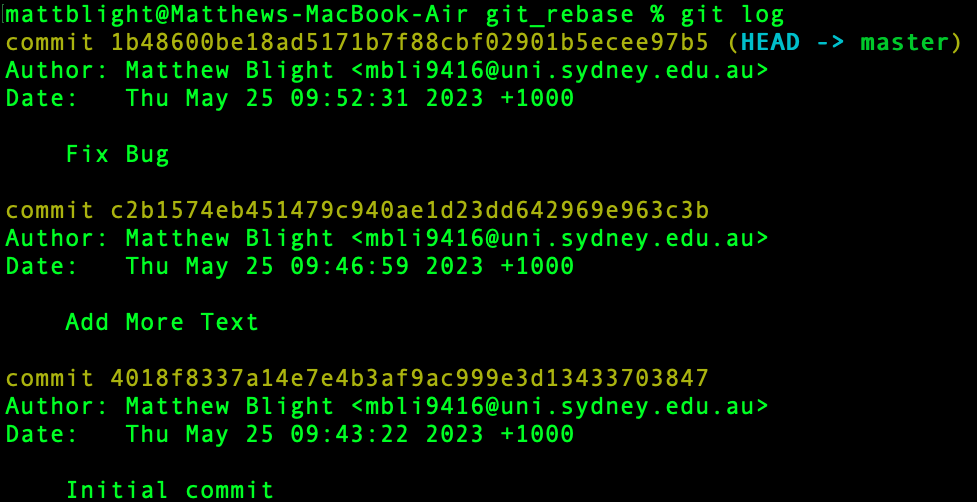
\includegraphics[width=\textwidth]{rebase1}

And our \verb|feature| branch log is below (note that the ‘Add More Text’ and ‘Fix Bug’ commits are not here):

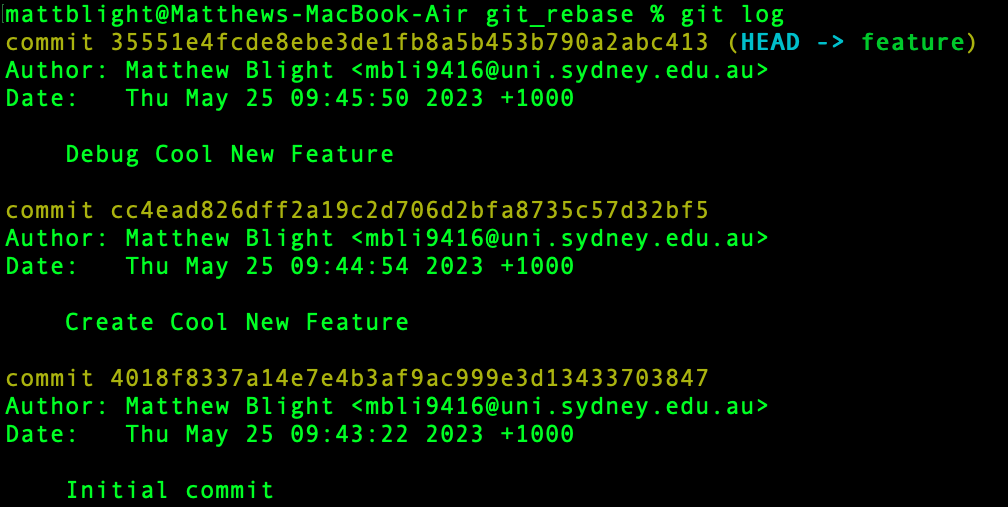
\includegraphics[width=\textwidth]{rebase2}

You realise that the new commits in \verb|master| are useful for your feature, but you don’t want to create a new merge commit in your \verb|feature| branch. Instead, you want it to seem like you were working on \verb|feature| from the latest \verb|master| commit. Here, you would use the command \verb|git rebase master|. This creates a new ‘base’ for the \verb|feature| branch, re-writing the commit history to show \verb|feature| branching off from the newest \verb|master| commit. The rebased log would look like this:

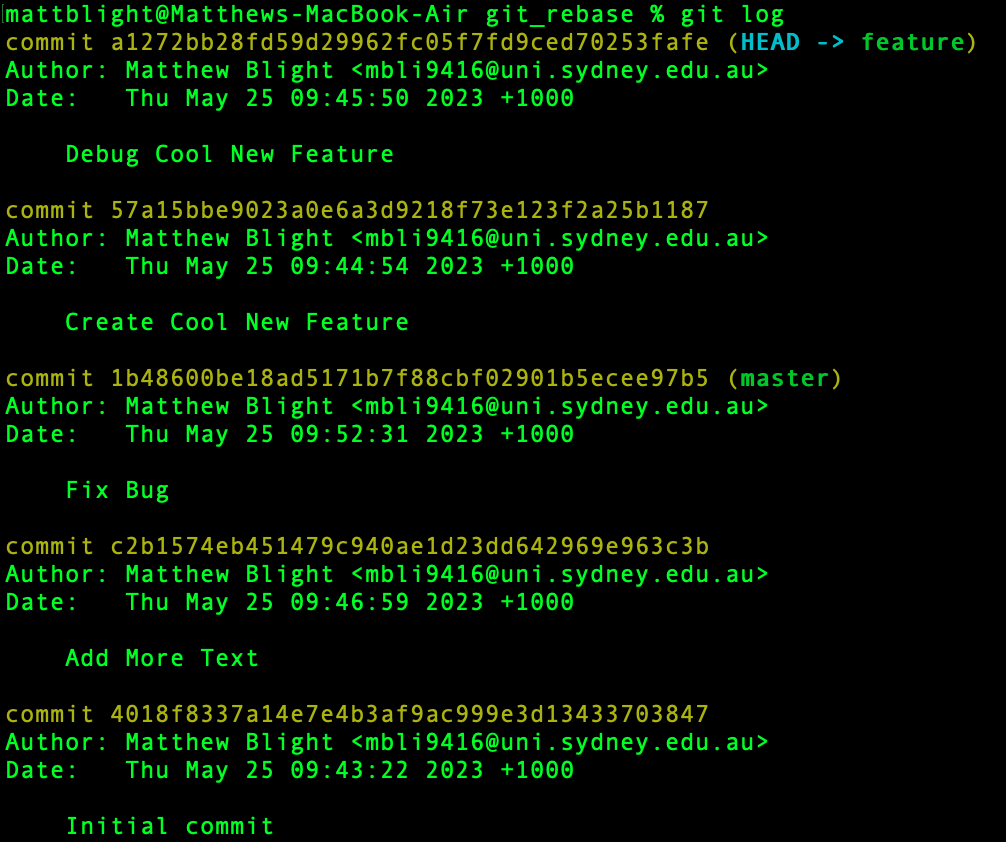
\includegraphics[width=\textwidth]{rebase3}

The \verb|git rebase| command is incredibly useful for keeping commit history clean and linear, rather than having multiple merge commits, which can look especially messy if the \verb|master| branch is very active. The main rule to remember with this command is to never use it on public branches, as re-writing commit history can make collaboration incredibly messy \cite{rebase}.

\subsubsection{Git: Ignoring Files \cite{ignore}}

Sometimes a project may have files that you don’t want to commit to a repository. These may be:

\begin{itemize}
	\item compiled code, such as \verb|.pyc| files
	\item hidden systems files, such as \verb|.DS_Store|
	\item files generated at runtime, such as \verb|.log|
\end{itemize}

While this problem could be solved by only staging the files needed, this can be extraneous and results in git showing that there are untracked files:

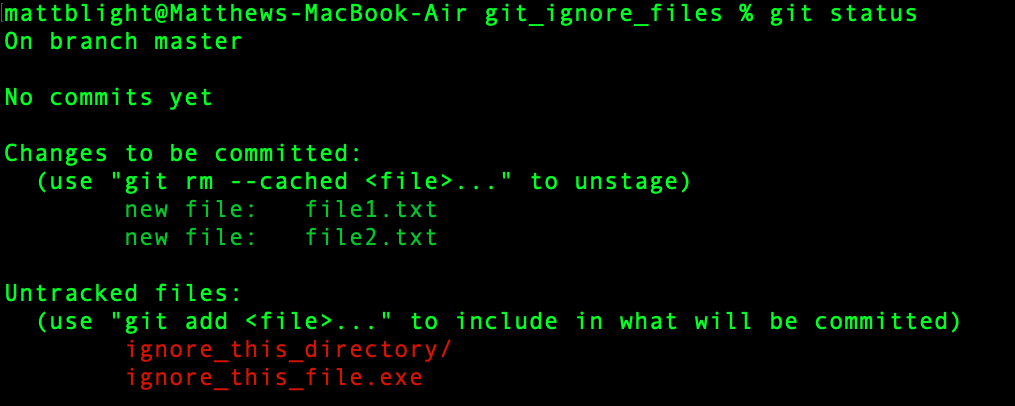
\includegraphics[width=\textwidth]{ignore1}

A better way of solving this problem is to create a file called \verb|.gitignore| at the root of the repository, which stores the names of files and directories that you want git to ignore. For our example, our \verb|.gitignore| file contains \verb|ignore_this_file.exe| and \verb|ignore_this_directory|: 

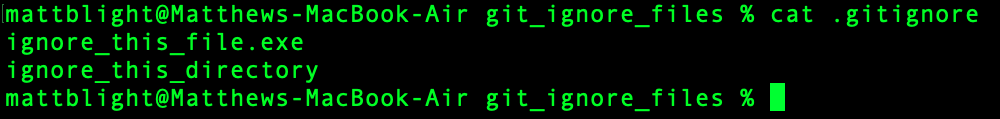
\includegraphics[width=\textwidth]{ignore2}

These files and directories will be automatically ignored when staging and committing, as seen below:

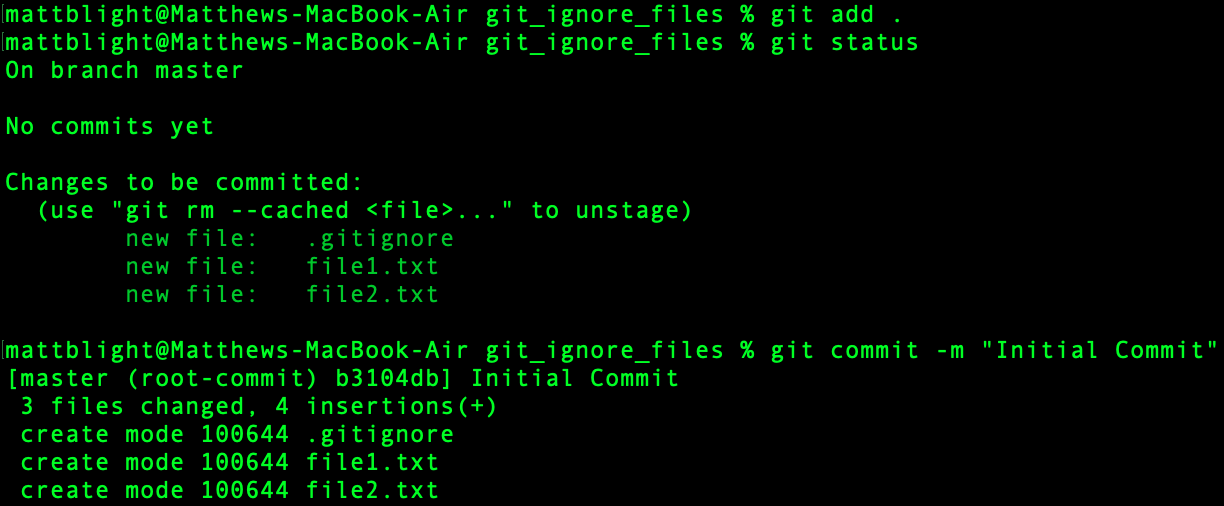
\includegraphics[width=\textwidth]{ignore3}

%=======================================================================================

\newpage


\subsubsection{\LaTeX\ : Footnotes and Margin Notes \cite{footnotes}}

Footnotes are a great way to provide extra information to the reader whilst keeping the main flow of the text clean and concise.\footnote{This is an example of a footnote.} Footnotes are easy to implement in LaTeX. Simply use the command \verb|\footnote{text}|, and your text will be automatically be placed at the bottom of the page.\footnote{Footnotes will automatically be numbered sequentially.}

Margin notes are a great way to exchange comments between authors in the editorial process, or otherwise to provide extra information to the reader. To insert a margin note, use the command \verb|\marginpar{margin note}|. \marginpar{Margin notes are inserted in the outside margin, starting from the line where it is defined.}

\subsubsection{\LaTeX\ : Creating New Environments}

Environments in LaTeX are useful for applying specific effects to sections of a document. There are a number of existing LaTeX environment, however it is useful to know how to create new environments. The basic syntax for defining a new environment is \verb|\newenvironment{<env-name>}[<n-args>][<default>]{<begin-code>}{<end-code>}|, where \verb|<env-name>| is the name of the new environment. \verb|<begin-code>| and \verb|<end-code>| is the LaTeX code to be applied at the beginning and end of the environment. \verb|<n-args>| can be used to define an environment with arguments, and \verb|<default>| can be used to define an environment with an optional argument. As an example, we can create a new environment called \verb|boldbox|, which puts text in a centered box and makes it bold. The environment definition would be:

\begin{verbatim}
\newenvironment{boldbox}
    {\begin{center}
    \begin{tabular}{|p{\textwidth}|}
    \hline\\
    \bfseries
    }
    { 
    \\\\\hline
    \end{tabular} 
    \end{center}
    }
\end{verbatim}

We can this use this just like any other LaTeX environment:

\begin{verbatim}
\begin{boldbox}
I want this text to be bold in a box!
\end{boldbox}
\end{verbatim}

Which results in:

\begin{boldbox}
I want this text to be bold in a box!
\end{boldbox}


%=======================================================================================

\newpage

\subsection{Advanced skills: \studB}

Explain your use of the advanced Git and \LaTeX\ features. 

\subsection{Advanced skills: \studC}

Explain your use of Git Forking and Special files and \LaTeX\ Floating Figures and Styling Sheets

\subsubsection{Git: Forking}

git forking doesn't have a specific command, but instead involves using the command line to clone the existing repository and disconnecting the codebase from previous committers using subcommand gh repo fork.  The steps to forking a git repository is to copy the git repo by cloning it to a new folder and removing any remote references to isolate the fork from the original codebase.  \cite{gitfork}  For example,  check an existing empty repository for its contents:

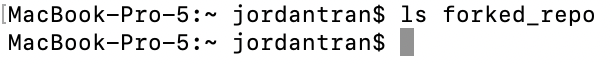
\includegraphics[width=\textwidth]{empty_fork}

Now clone the the existing repository into the empty directory using the command line git clone 

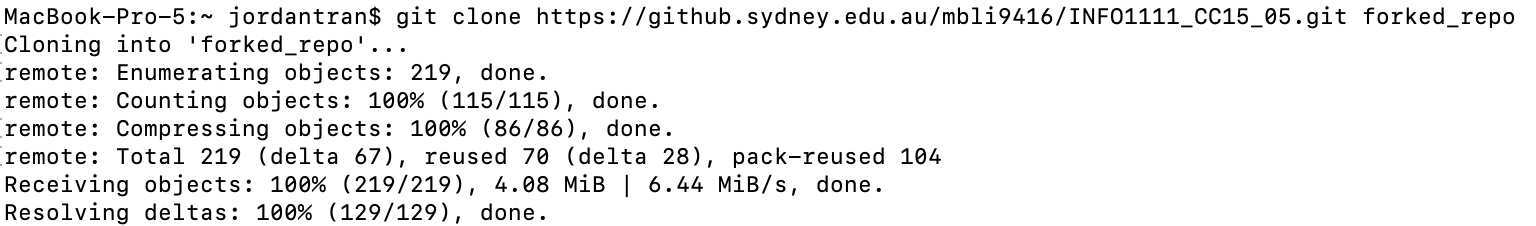
\includegraphics[width=\textwidth]{cloning}

Now check the contents of the new repository to see if original has been forked:

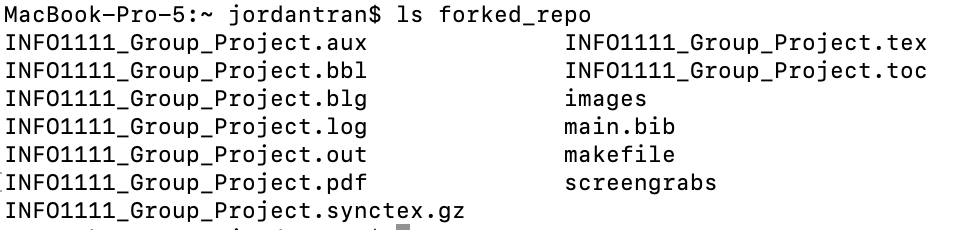
\includegraphics[width=\textwidth]{fork_repo}

Git forking is common practice allowing developers to propose and experiment with bugs without messing up the original repository so that once they are satisfied with the outcomes,  they can submit a pull request to the original repository for a potential inclusion of the updated and experimented code. 

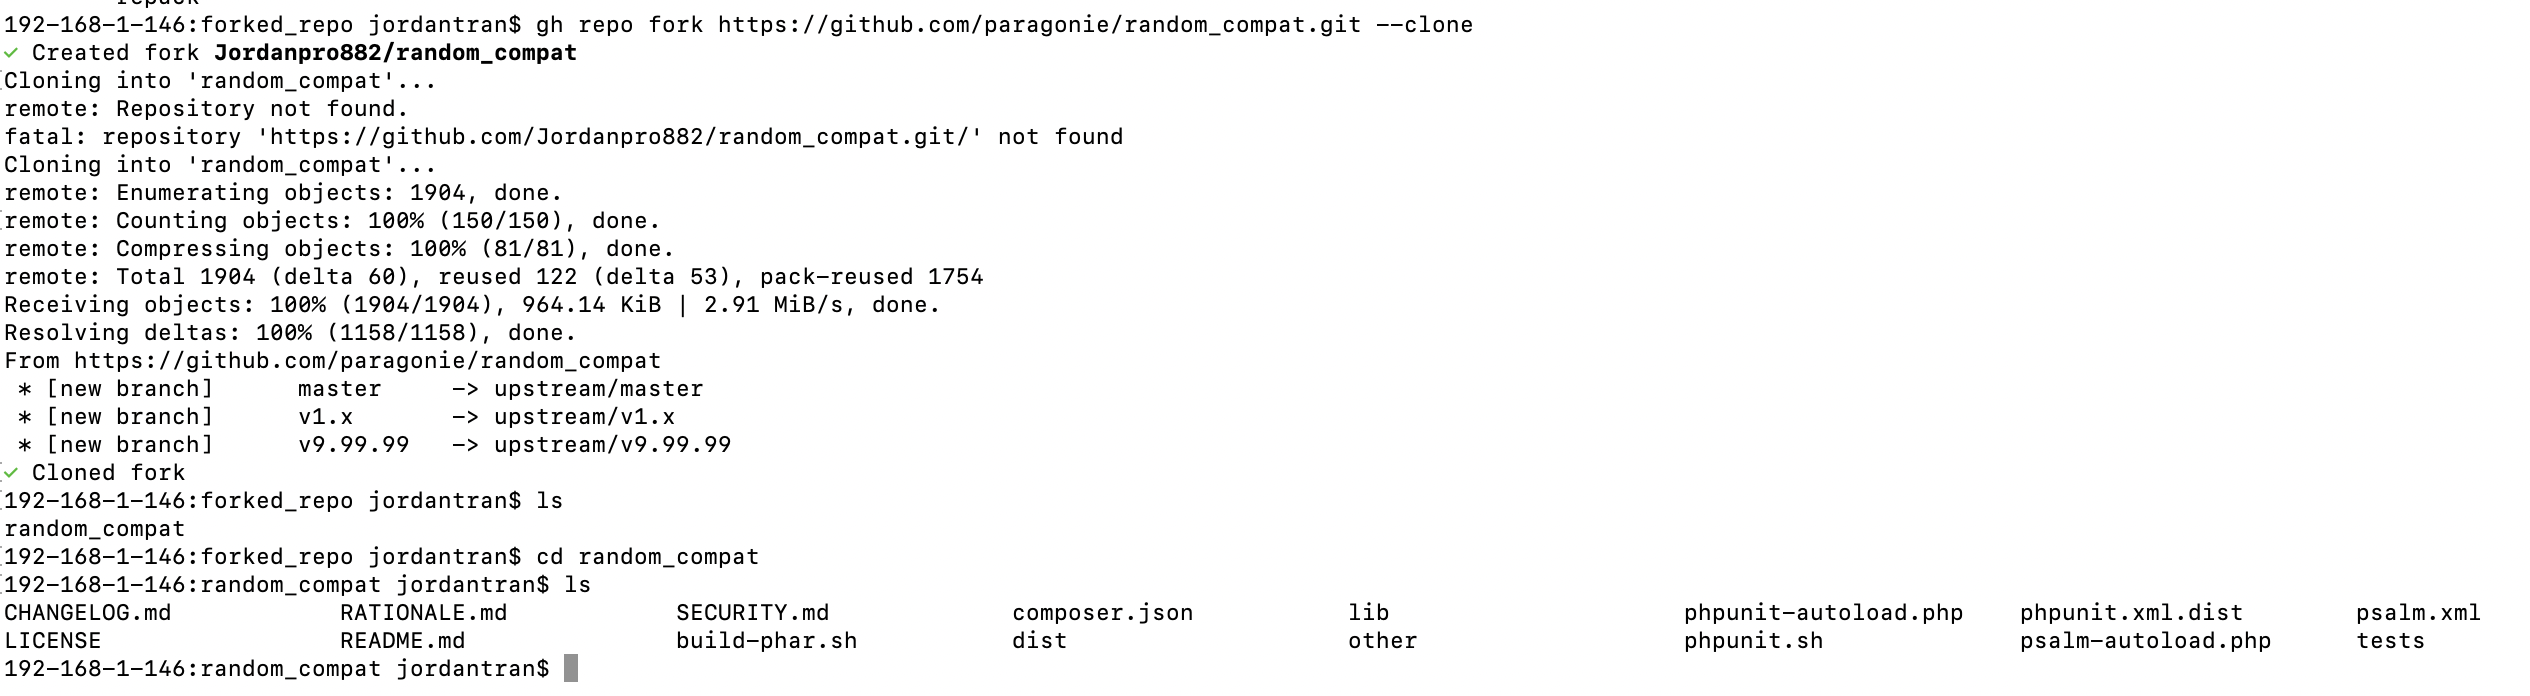
\includegraphics[width=\textwidth]{git_fork}

Here I used the gh repo fork [repository] command to fork from the existing repository 'random compat' to create my own copy of it in a remote location so that I can add independent changes to it myself. I then checked the contents of the remote location to see if it has been sucessfully forked.

\subsubsection{Git: Special File}

Git Special Files are files that have specific properties and purposes within Git and are often used to customise the behaviour and configuration of the repository enhancing collaboration and workflows through git. There are 4 commonly recognised special files in git being .gitignore .gitattributes .gitmodules and .gitkeep \cite {medium} . 

\subsubsection{.gitignore files \cite{pluralsight}:}

When committing there may be files that developers might not want to commit, so they use the .gitignore special so that it lets git knows that these files shouldn't be added to the repository and ignore them. For example you set a .gitignore file by using the command lines:

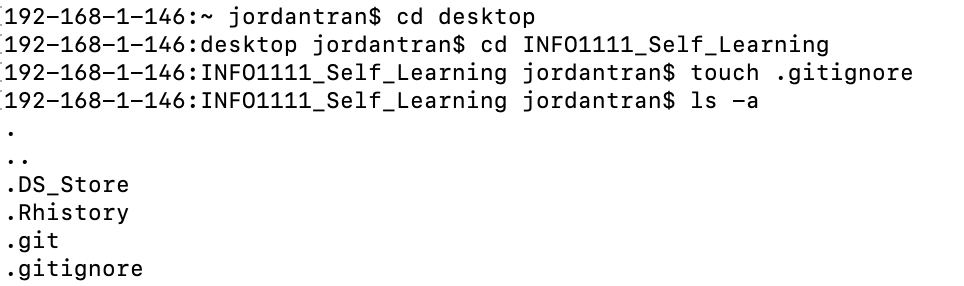
\includegraphics[width=\textwidth]{create_gitignore}

now type in 'open .gitignore' into the command line to open the special file and then write the file/directory name that you want to avoid committing into the git repository

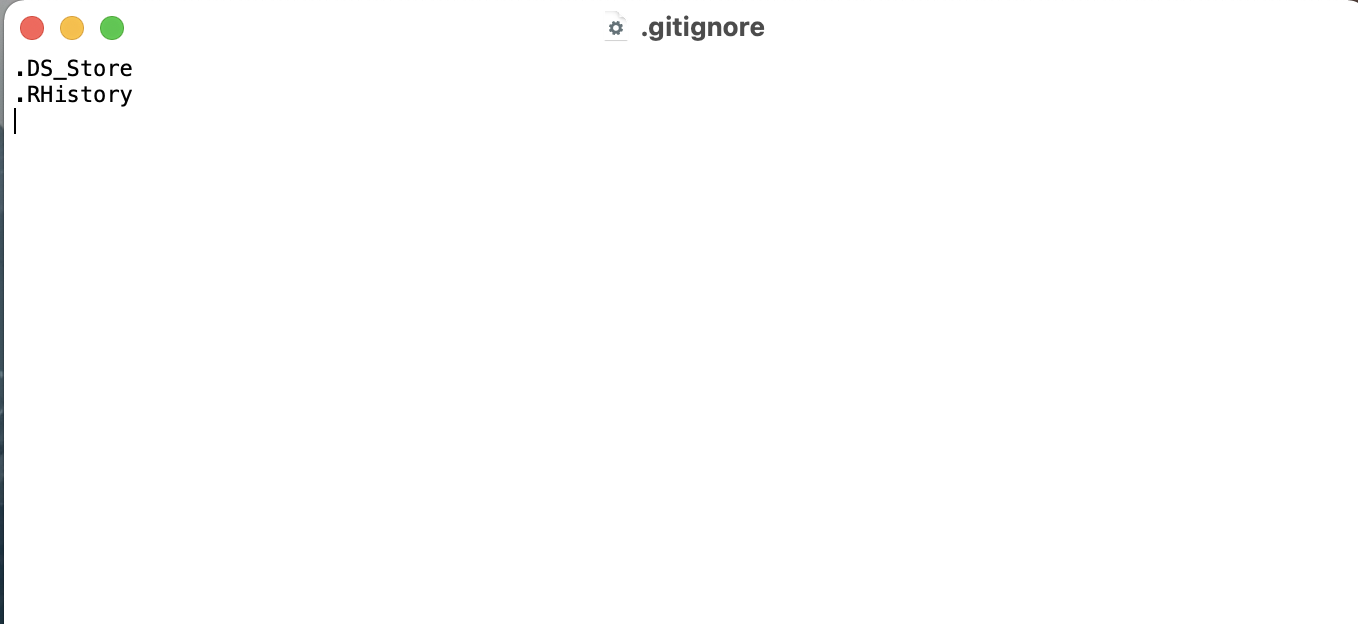
\includegraphics[width=\textwidth]{ignore_contents}

Now make a new commit called git add .gitignore to add the contents of gitignore to the git repository and push it so that in the future it will now know what to avoid adding.

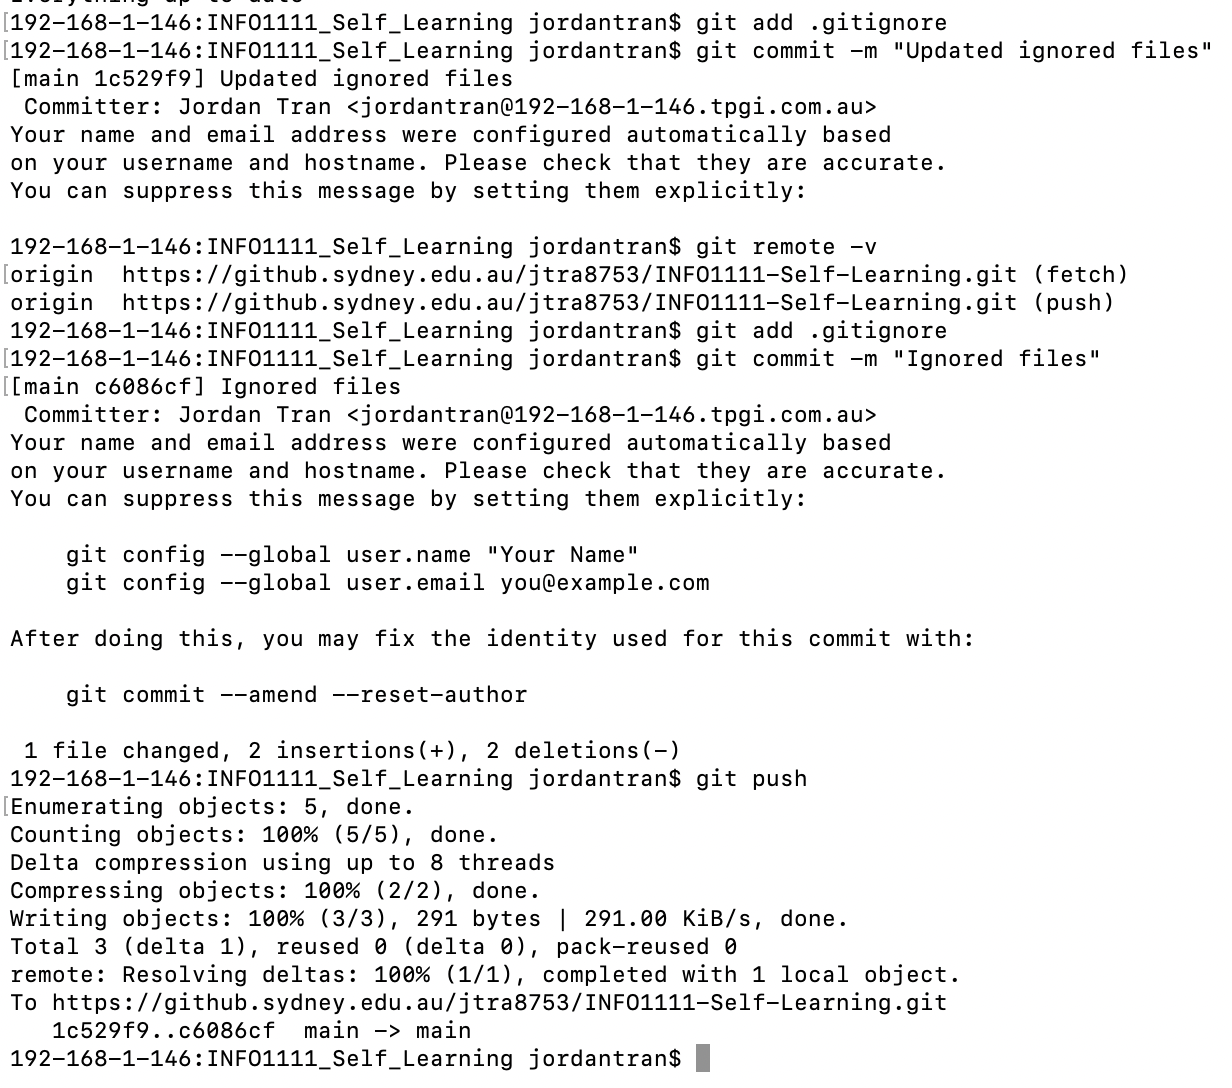
\includegraphics[width=\textwidth]{ignore_push}

\subsubsection{.gitattribute files\cite{codepath}}

The gitattributes file is a useful special file that alters the configuration of git repositories. For instance, it tells git how to treat certain files and projects.  For instance, the command *.pbxproj binary merge=union sets projects to binary so that git will treat them as binary and avoid merging them with other text files.  Creating a gitattributes file and checking its existence goes as:

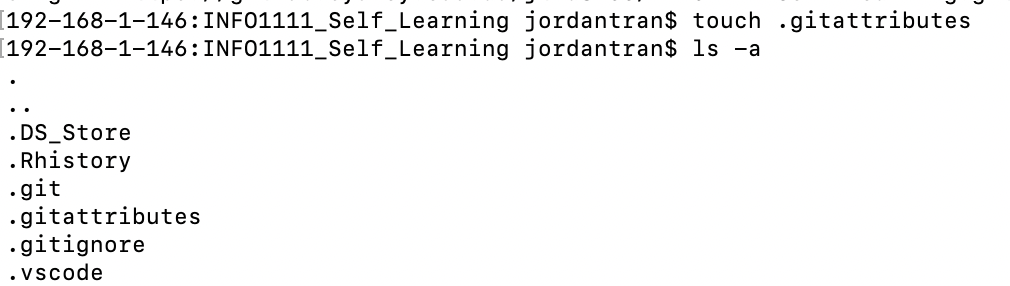
\includegraphics[width=\textwidth]{create_gitattributes}

Now open gitattributes file and add contents:


\includegraphics[width=\textwidth]{gitattributes_contents}

Then push the .gitattribute file into the directory

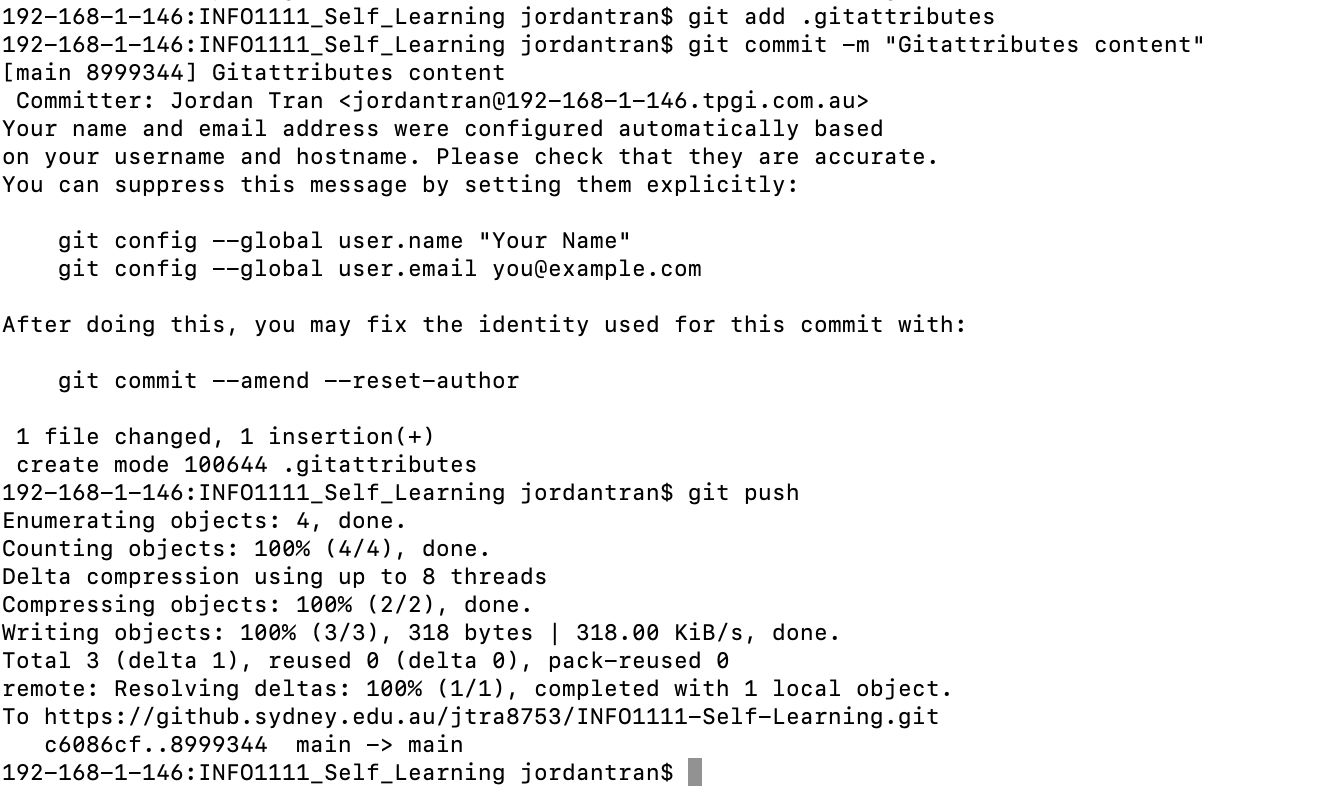
\includegraphics[width=\textwidth]{add_gitattributes}

\newpage

\subsubsection{LaTeX: Floating Figures\cite{WikiBooks}}

Floating figures are useful features in LaTeX that are not part of the normal stream of text, but are seperate entities positioned anywhere on the page that the user describes hence the name, 'float.' There are multiple specifiers that all have different properties for the inputted entity.

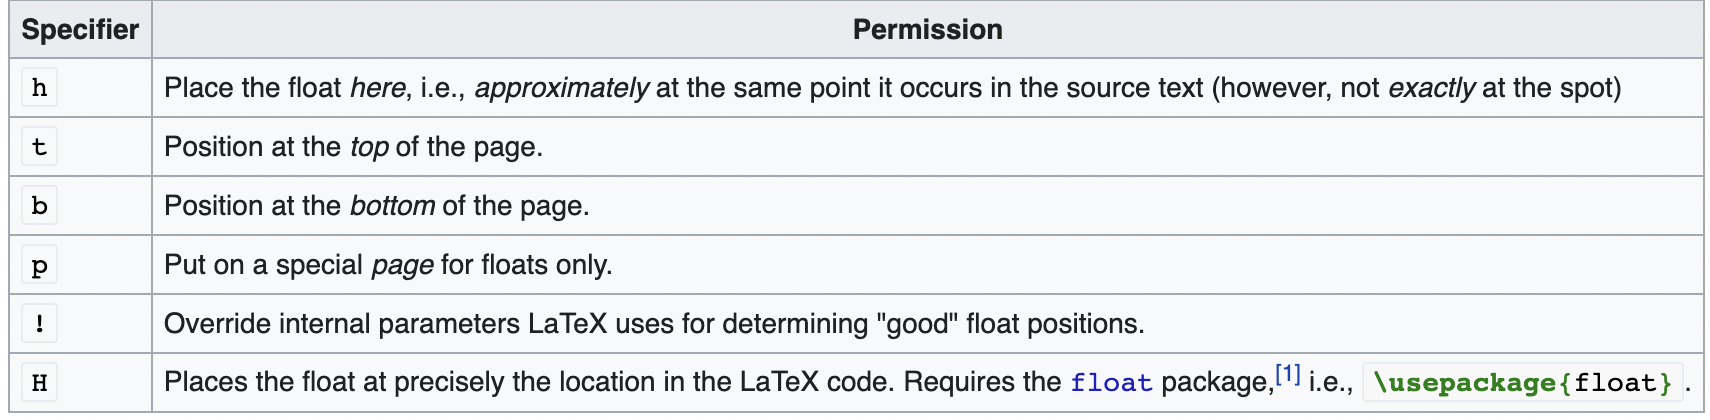
\includegraphics[width=\textwidth]{float_table}

The syntax to applying a floating figure is <{figure}[placement specifier]>.

Floats can be specifically useful in which if a figure causes the figure to run off into a new page and breaking the current page,  you can use floats to avoid this issue.  If you scroll down to the bottom of the current page and top of the next page,  you will see a floating figure that has the placement specifier being set as 'b'.

\begin{figure}[b]
...bottom floating figure here! ...
The main advantage of using floats is to avoid wasting large empty spaces due to a table or image not fitting.
\end{figure}

\begin{figure}[t ]
...top floating figure here! ...
Users would commonly use this if there is not enough space to fit the remainder of the current page and would float this figure to the next and will the current page with body text.
\end{figure}

\subsubsection{LaTeX: Editing Style Sheets \cite{stylesheets}}
\pagestyle{fancy}
Style sheets in LaTeX typically refer to style files or packages that contain predefined formatting instructions that shape the appearance and layout of a LaTeX document.  Editing style sheets allow precise control over the visual representation of the LaTeX documents and can greatly enhance readability.  Style packages usually have an extension .sty and are included in LaTeX through the syntax <usepackage>.

Examples:

Using one of the predefined packages in this report, 'fancyhdr' I have already adjusted the layout of this page using the syntax <pagestyle[fancy]> to give a professional look to my report.  Moreover, I can include extra footers into the pages as seen at the bottom of this page to the left and right.  Moreover, at the top with the included header for the fancy layout, I have also added in a header using the syntax <fancyhead[C]large-text>

\fancyhead[C]{\large HEADER!!!}

\lfoot{left footer}

\rfoot{right footer}

\newpage

\lfoot{}
\rfoot{}

\pagestyle{fancy}

\subsection{Advanced skills: \studD}

Explain your use of the advanced Git and \LaTeX\ features. 



%=======================================================================================

\newpage

\section{Level D: Evolution of skills}

Level D focuses on understanding how professional practice might evolve in the future. Most students in this unit are likely to be at or near the start of your degree, and so it might be anywhere from 3 to 5 years before you really start working in industry full-time -- and the technology and ways in which people use them can change significantly in that time. 

Your answer to this section you should address the following (Target = $\sim$500 words):
\begin{enumerate}
	\item Describe what you believe will be the biggest change in the next 5 years in the tools or technologies that are being actively used in industry practice (in your selected major);
	\item Revisit the SFIA framework~\cite{sfia} from level A, and identify the one skill that you believe will have the biggest increase in terms of importance over the next 5 years. You should justify your choice.
\end{enumerate}


\subsection{Evolution of \majA: \studA}

Your text goes here

\subsection{Evolution of \majB: \studB}

Your text goes here

\subsection{Evolution of \majC: \studC}

Your text goes here

\subsection{Evolution of \majD: \studD}

Your text goes here



%=======================================================================================

\newpage

\bibliographystyle{IEEEtran}
\bibliography{main}

\end{document}
\end{report}
